%Capitulo 5, presentación 21
\begin{frame}{Valor menos restrictivo}
    Dada una variable, escoger el valor menos restrictivo:
    \\
    \qquad el que descarta la menor cantidad de valores en las variables restantes
    \\
    \noindent\begin{minipage}{0.6\textwidth}% adapt widths of minipages to your needs
		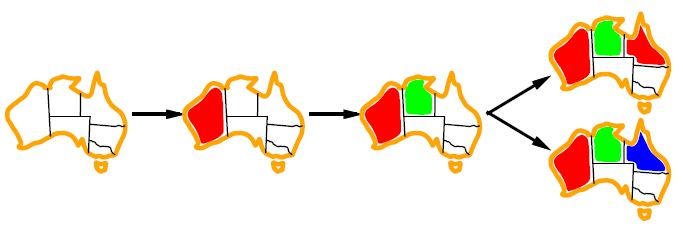
\includegraphics[scale=.45]{images/21_graph.JPG}
	\end{minipage}%
	\hfill%
	\begin{minipage}{0.33\textwidth}\raggedright
		{\small
				Permite 1 valor para SA
				\\
				\quad
				\\
				\quad
				\\
				Permite 0 valores para SA
		}
	\end{minipage}
	\\
    La combinación de estas heurísticas hace factibles 1000 reinas
\end{frame}